\documentclass[12pt,a4paper]{article}
\usepackage[MeX]{polski}
\usepackage[utf8]{inputenc}
\usepackage{listings}
\usepackage{graphicx}
\usepackage{fancyvrb}
\usepackage{tabularx}
\usepackage{geometry}
\usepackage{multirow}
\usepackage{amsmath}
\usepackage[hidelinks]{hyperref}
\usepackage{float}
\usepackage{color}

\geometry{
 a4paper,
 total={170mm,257mm},
 left=20mm,
 top=20mm,
}

\lstset{
frame = single,
breaklines,
basicstyle = \small,
language = C
}

\author{Paweł~Taborowski, Yurii~Vyzhha}
\title{Systemy Wbudowane \\Odtwarzacz plików dźwiękowych na STM32F407\\Sprawozdanie}
\begin{document}
  \maketitle
W ramach projektu na Systemy Wbudowane postanowiliśmy zrealizować odtwarzacz muzyczny na płytce  \emph{STM32F4 Discovery}. Pierwotna wersja projektu miała za zadanie odtwarzanie plików \emph{WAVE}, po czym zamierzaliśmy rozbudować projekt tak, by obsługiwał pliki \emph{MP3}.

Oprogramowanie naszego odtwarzacza jest uruchamiane na systemie operacyjnym czasu rzeczywistego \textit{FreeRTOS}.

\section{STM CubeMX}
Pracę zaczęliśmy od wygenerowania projektu w programie \emph{STM CubeMX}. Program ten służy do generowania kodu startowego projektu, uwzględniającego wykorzystywane peryferia, biblioteki (np. \textit{FatFS}) i interfejsy.

Konfiguracja naszego projektu wygląda następująco:

\begin{figure}[H]
 \centerline{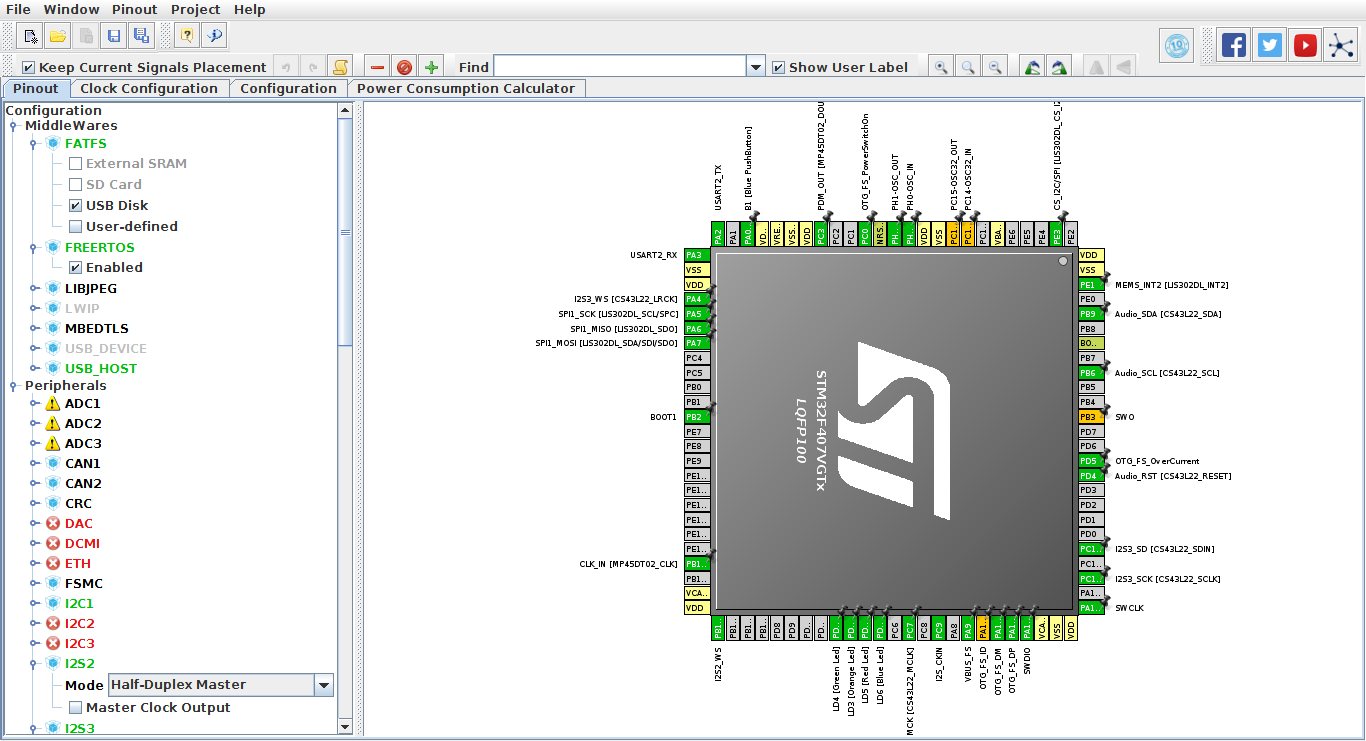
\includegraphics[width=\textwidth]{img/img1}}
 \caption{Konfiguracja \emph{FatFS}, \emph{FreeRTOS}, \emph{USB Host}, \emph{I2C1}, \emph{I2S2}}
 \label{img1}
\end{figure}

\begin{figure}[H]
 \centerline{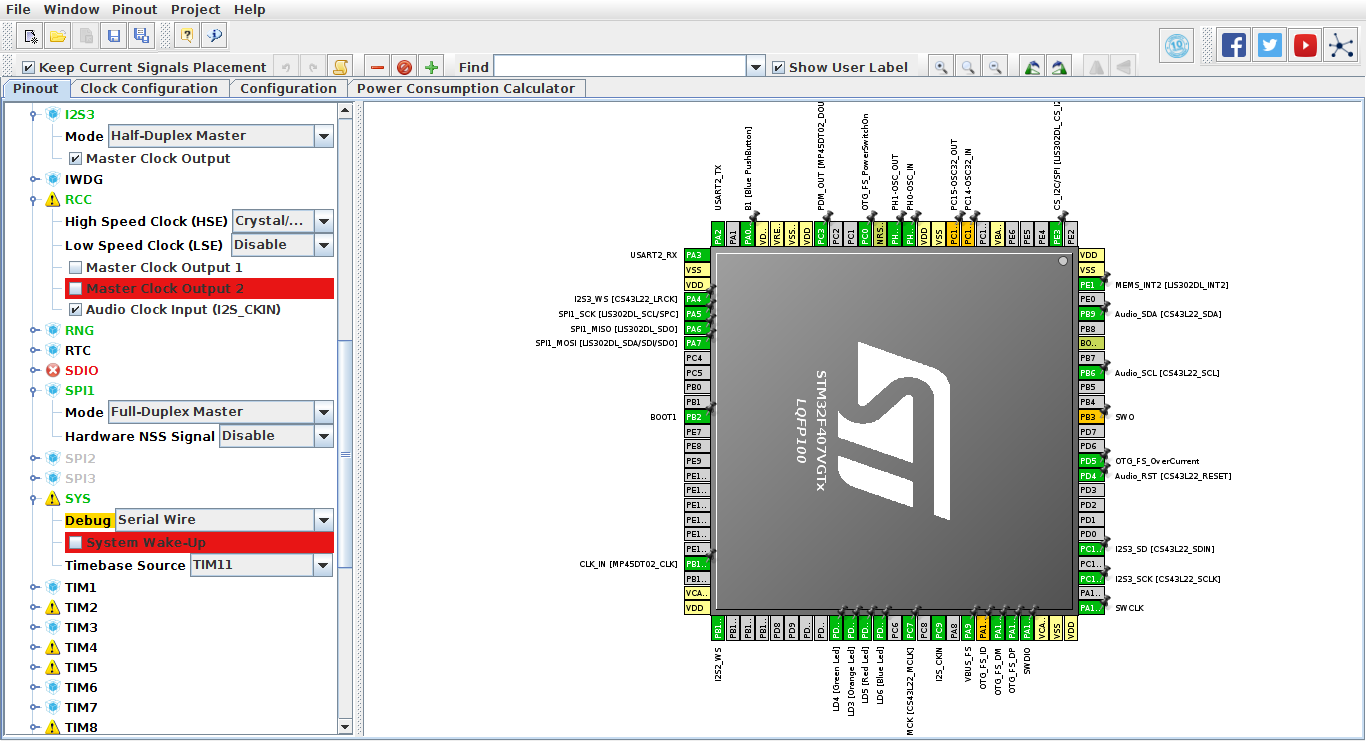
\includegraphics[width=\textwidth]{img/img2}}
 \caption{Konfiguracja \emph{I2S3}, \emph{RCC}, \emph{SPI1}, \emph{SYS}}
 \label{img2}
\end{figure}

\begin{figure}[H]
 \centerline{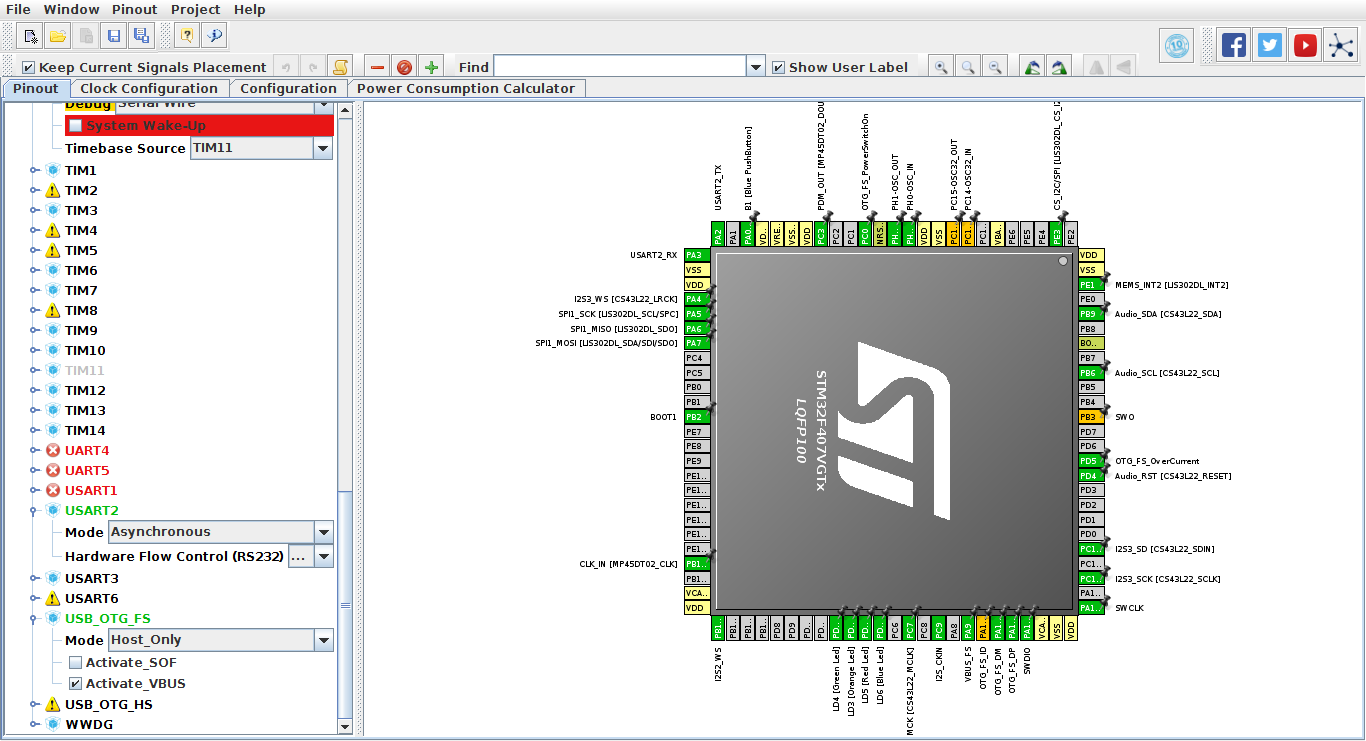
\includegraphics[width=\textwidth]{img/img3}}
 \caption{Konfiguracja \emph{USART2}, \emph{USB OTG FS}}
 \label{img3}
\end{figure}

\begin{figure}[H]
 \centerline{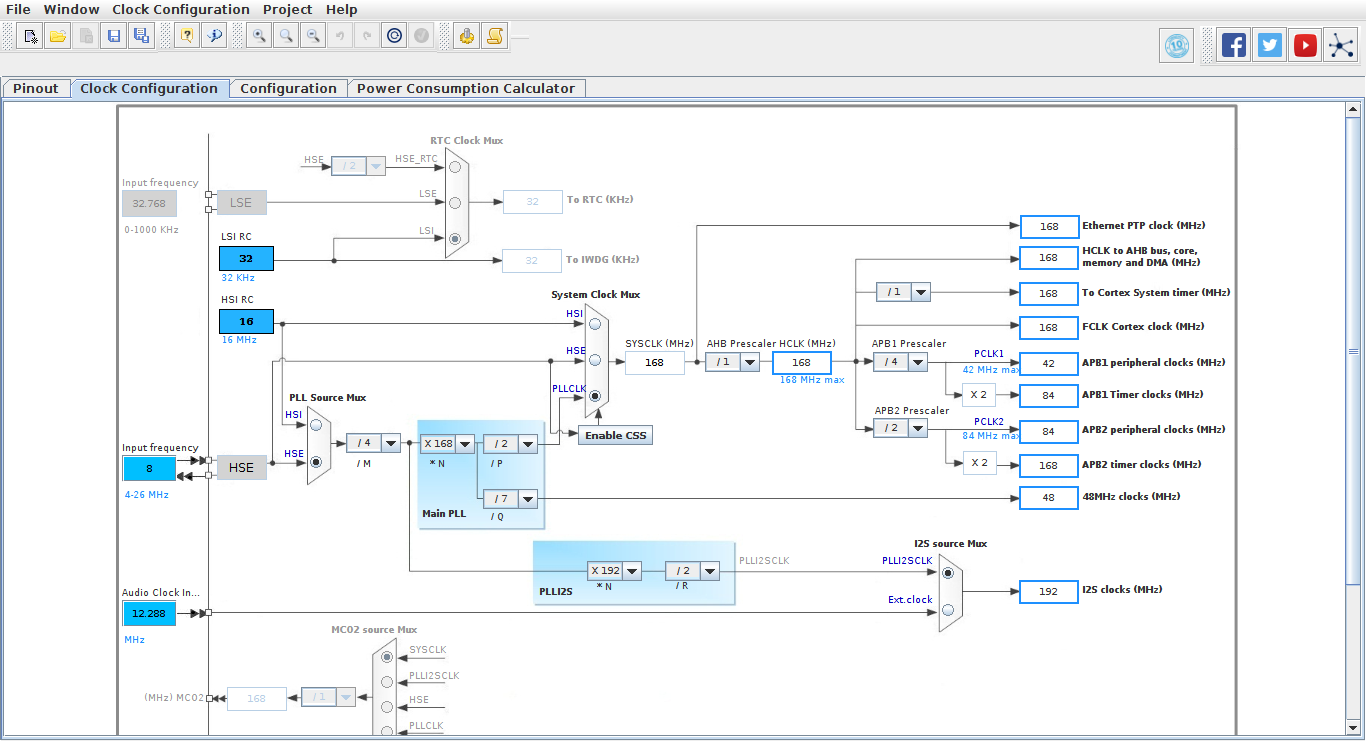
\includegraphics[width=\textwidth]{img/img4}}
 \caption{Konfiguracja zegara}
 \label{img4}
\end{figure}

\begin{figure}[H]
 \centerline{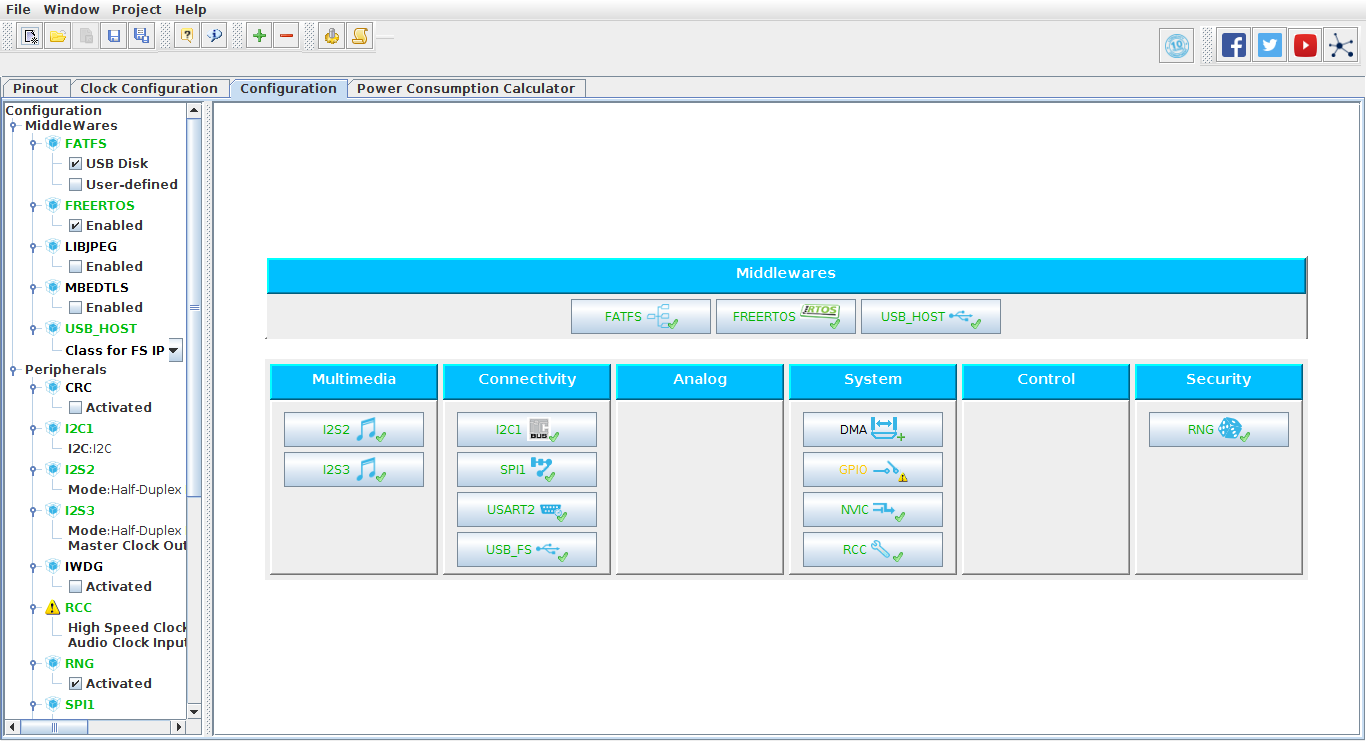
\includegraphics[width=\textwidth]{img/img5}}
 \caption{Podsumowanie konfiguracji}
 \label{img5}
\end{figure}

\section{Środowisko programistyczne}
Do rozwijania naszego projektu wykorzystywaliśmy środowisko \emph{GNU MCU Eclipse}. Wymagało ono wstępnej konfiguracji -- ustawienie ścieżek do kompilatora, debuggera oraz modyfikacji pliku \texttt{Makefile}.

\begin{figure}[H]
 \centerline{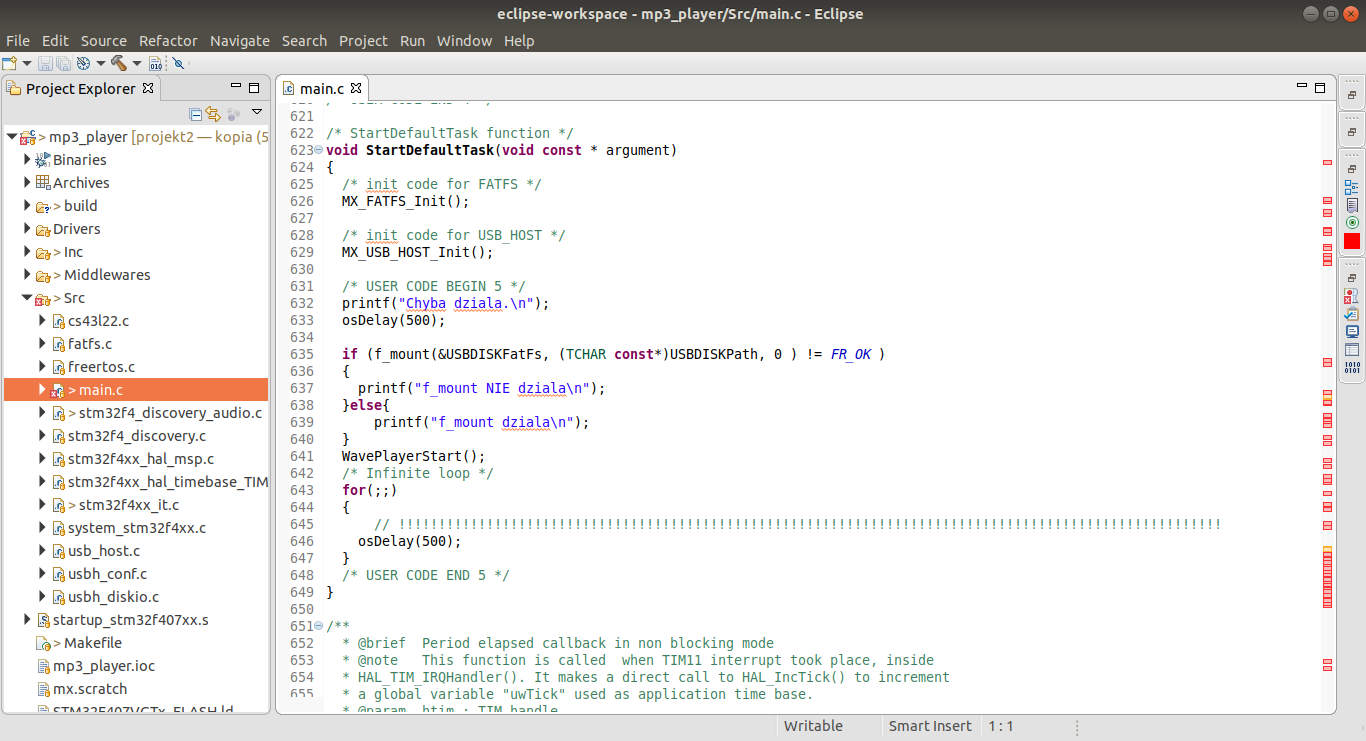
\includegraphics[width=\textwidth]{img/img6}}
 \caption{Środowisko programistyczne \emph{Eclipse}}
 \label{img6}
\end{figure}

\section{Procedura debugowania}
Płytkę STM32F4 Discovery podłączaliśmy do komputera za pomocą USB. Urządzenie było widoczne między innymi jako emulowany port szeregowy COM, co umożliwiało debugowanie przy użyciu programu \emph{ExtraPUTTY}. Wyświetlał on komunikaty, które umieszczaliśmy w kodzie programu przy pomocy funkcji \texttt{printf()}. Aby mogła ona działać, zaimplementowaliśmy poniższe funkcje:

\begin{lstlisting}
/* For printf */
#define PRINTF_UART huart2
#define AUDIO_BUFFER_SIZE 4096

extern UART_HandleTypeDef PRINTF_UART;

static void print_chr(char chr) {
    HAL_UART_Transmit(&PRINTF_UART, (uint8_t * ) & chr, 1, 1000);
}

ssize_t _write_r(struct _reent *r, int fd, const void *ptr, size_t len) {
    int cntr = len;
    char *pTemp = (char *) ptr;
    while (cntr--) print_chr(*pTemp++);
    return len;
}
\end{lstlisting}

\section{\emph{Wave Player} -- przegląd kodu}

\subsection{Założenia projektu}
Ta wersja projektu ma za zadanie odtwarzanie pliku \emph{WAVE} o danej nazwie z podłączonej do płytki przez USB pamięci flash. Kolejne kroki wykonywane przez program to:
\begin{itemize}
 \item montowanie systemu plików,
 \item otwieranie pliku muzycznego,
 \item wczytywanie początku pliku do bufora,
 \item rozpoczęcie odtwarzania danych z bufora,
 \item uzupełnianie bufora w reakcji na przerwania,
 \item kończenie odtwarzania.
\end{itemize}

\subsection{Default Task (\emph{FreeRTOS})}

\begin{lstlisting}
/* StartDefaultTask function */
void StartDefaultTask(void const *argument) {
    /* init code for FATFS */
    MX_FATFS_Init();

    /* init code for USB_HOST */
    MX_USB_HOST_Init();

    /* USER CODE BEGIN 5 */
    osDelay(500);

    if (f_mount(&USBDISKFatFs, (TCHAR const *) USBDISKPath, 0) != FR_OK) {
        printf("f_mount FAILED\n");
    } else {
        printf("f_mount SUCCEDED\n");
        WavePlayerStart();
    }
    /* Infinite loop */
    for (;;) {
        osDelay(500);
    }
    /* USER CODE END 5 */
}
\end{lstlisting}

W głównym zadaniu systemu operacyjnego inicjalizujemy biblioteki \emph{FatFS} i \emph{USBhost}, a następnie montujemy system plików. Jeżeli ta operacja się powiodła, to przystępujemy to dalszej pracy. \newpage

\subsection{Funkcja \texttt{void WavePlayerStart(void)}}

\begin{lstlisting}
void WavePlayerStart(void) {
    UINT bytesread = 0;
    char *wavefilename = WAVE_NAME;
    WAVE_FormatTypeDef waveformat;
    /* Open the Wave file to be played */
    int status;
    if ((status = f_open(&FileRead, wavefilename, FA_READ)) != FR_OK) {
        printf("Failed to open the file %d\n", status);
    } else {
        printf("File open successful\n");
        /* Read sizeof(WaveFormat) from the selected file */
        f_read(&FileRead, &waveformat, sizeof(waveformat), &bytesread);

        /* Set WaveDataLenght to the Speech Wave length */
        WaveDataLength = waveformat.FileSize;

        /* Play the Wave */
        WavePlayBack(waveformat.SampleRate);
    }
}
\end{lstlisting}

W tej funkcji próbujemy otworzyć plik o zadanej nazwie. Jeśli nam się to udało, to wczytujemy nagłówek tego pliku do struktury przechowywanej w zmiennej \texttt{waveformat}. Na podstawie danych otrzymanych z nagłówka ustawiamy wartości odpowiednich zmiennych i przystępujemy do właściwego odtwarzania pliku.

\subsection{Funkcja \texttt{void WavePlayBack(uint32\_t AudioFreq)}}

\begin{lstlisting}
void WavePlayBack(uint32_t AudioFreq) {
    UINT bytesread = 0;

    /* Initialize Wave player (Codec, DMA, I2C) */
    if (BSP_AUDIO_OUT_Init(OUTPUT_DEVICE_AUTO, Volume, AudioFreq) != 0) {
        Error_Handler();
    }

    /* Get Data from USB Flash Disk */
    f_lseek(&FileRead, 0);
    f_read(&FileRead, &Audio_Buffer[0], AUDIO_BUFFER_SIZE, &bytesread);
    AudioRemSize = WaveDataLength - bytesread;

    /* Start playing Wave */
    BSP_AUDIO_OUT_Play((uint16_t*) &Audio_Buffer[0], AUDIO_BUFFER_SIZE);

    /* Check if the device is connected.*/
    while ((AudioRemSize != 0) && (Appli_state != APPLICATION_IDLE)) {
        bytesread = 0;

        if (buffer_offset == BUFFER_OFFSET_HALF) {
            f_read(&FileRead,
                   &Audio_Buffer[0],
                   AUDIO_BUFFER_SIZE / 2,
                   (void *) &bytesread);

            buffer_offset = BUFFER_OFFSET_NONE;
        }

        if (buffer_offset == BUFFER_OFFSET_FULL) {
            f_read(&FileRead,
                   &Audio_Buffer[AUDIO_BUFFER_SIZE / 2],
                   AUDIO_BUFFER_SIZE / 2,
                   (void *) &bytesread);

            buffer_offset = BUFFER_OFFSET_NONE;
        }

        if (AudioRemSize > (AUDIO_BUFFER_SIZE / 2)) {
            AudioRemSize -= bytesread;
        } else {
            AudioRemSize = 0;
        }
    }

    /* Stop playing Wave */
    WavePlayerStop();

    /* Close file */
    f_close(&FileRead);
}
\end{lstlisting}

W funkcji \texttt{WavePlayBack(uint32\_t AudioFreq)} najpierw inicjalizujemy kodek, \emph{DMA} oraz \emph{I2C}. Następnie wczytujemy pierwszą porcję danych audio do bufora i odtwarzamy ją funkcją \texttt{BSP\_AUDIO\_OUT\_Play()}. Dopóki nie~odtworzymy całego utworu, w miarę potrzeb doczytujemy porcje pliku do bufora.

Po skończonym odtwarzaniu, zamykamy plik.

\section{\emph{MP3 Player}}

Gdy skończyliśmy pracę nad odtwarzaczem plików \emph{WAVE}, zaczęliśmy rozszerzać funkcjonalność naszego programu o możliwość odtwarzania plików \emph{MP3}.

Zadanie to miało zostać zrealizowane w następny sposób:
\begin{itemize}
 \item dekodowanie kolejnych ramek pliku \emph{MP3} przy pomocy biblioteki \texttt{Helix} do formatu takiego jak w pliku \emph{WAVE},
 \item odtwarzanie otrzymanych fragmentów za pomocą już istniejącej funkcjonalności odtwarzania plików \emph{WAVE}.
\end{itemize}

Kod biblioteki \texttt{Helix} dołączyliśmy do naszego projektu i skonfigurowaliśmy jego kompilację razem z projektem.

Dekodowanie ramek \texttt{MP3} odbywa się w funkcji \texttt{int MP3Decode(HMP3Decoder hMP3Decoder, unsigned char **inbuf, int *bytesLeft, short *outbuf, int useSize)}. Dekodowane \\ dane są zwracane przez zmienną \texttt{outbuf}.

Projektu nie udało nam się ukończyć. W trakcie prac poznaliśmy złożony proces dekodowania i odtwarzania plików \emph{MP3} o zmiennej długości ramki, którego nie udało nam się w pełni zaimplementować.

\end{document}
